\documentclass[journal]{IEEEtran}
\usepackage{amsmath,amssymb,amsthm,graphicx,booktabs,subcaption,algorithm,algpseudocode,hyperref,cleveref}
% Notation for the whole paper. Do not redefine these in section files.
\newcommand{\norm}[1]{\left\lVert #1 \right\rVert}
\newcommand{\score}{s_\theta}
\newcommand{\E}{\mathbb{E}}
\newcommand{\R}{\mathbb{R}}
\newcommand{\anchor}{\tilde{g}}
\newcommand{\kap}{\kappa}
\newcommand{\xhat}{\hat{x}_0}
\newcommand{\meas}{y}
\newcommand{\fwd}{A}
\DeclareMathOperator*{\argmin}{arg\,min}
\DeclareMathOperator{\clip}{clip}
\newtheorem{theorem}{Theorem}
\newtheorem{lemma}{Lemma}
\newtheorem{assumption}{Assumption}
\newtheorem{corollary}{Corollary}


\title{Score Anchoring for Diffusion Posterior Sampling: Theory, Samplers and a Study Across Six Inverse Problems}
\author{Aurelio Vantreight,~\IEEEmembership{Member,~IEEE,} Ilse Marrowfield, Teodor Quenzel, and Beatriz Olamide-Farrant%
\thanks{A. Vantreight and I. Marrowfield are with the Institute of Computational Imaging, Ravensbourne University. T. Quenzel is with Halden Research. B. Olamide-Farrant is with the Department of Radiology, St. Cuthbert's Hospital.}}

\begin{document}
\maketitle

\begin{abstract}
Diffusion posterior sampling drifts when the guidance gradient and the learned score disagree at low noise levels. We introduce score anchoring, a single scalar correction that keeps the guided trajectory within a trust region of the prior score, and extend our earlier conference result in three directions. First, we prove that the anchored update is a contraction under a mild smoothness assumption on the score. Second, we show that the same rule transfers to DDIM, predictor--corrector and stochastic samplers without retuning. Third, we evaluate on six inverse problems including sparse-view CT, accelerated MRI, deblurring, inpainting, super-resolution and phase retrieval, where anchoring holds a 1.8 dB PSNR margin over five baselines across noise levels up to $\sigma = 0.3$ with no extra network evaluations.
\end{abstract}

\begin{IEEEkeywords}
Diffusion models, inverse problems, posterior sampling, computational imaging, trust region.
\end{IEEEkeywords}

\section{Introduction}
\label{sec:intro}
\IEEEPARstart{R}{econstructing} an image from incomplete measurements is ill-posed unless the prior closes the gap left by the forward operator~\cite{okonkwo2021,lindqvist2022}. Diffusion models are now the prior of choice for this role~\cite{ho2020ddpm,song2021sde,dhariwal2021}, but guided sampling can wander far from the data manifold when the likelihood term dominates~\cite{morales2023,chung2023dps}. We ask a narrow question: how far may the guidance move a sample before the score stops being trustworthy?

Our conference paper~\cite{vantreight2025anchor} answered this with score anchoring, a clip on the guidance gradient relative to the prior score. That paper studied two tasks, one sampler and a single noise range. Reviewers and later users raised three questions that this article answers. Does the rule have a convergence guarantee? Does it survive a change of sampler? Does it hold up on tasks whose forward operators are nonlinear or ill-conditioned in a different way from tomography?

\subsection{Contributions}
\label{sec:contributions}
\begin{itemize}
  \item A contraction result (\cref{thm:contraction}) showing that the anchored update shrinks the distance to the posterior mode under \cref{ass:smooth}.
  \item A sampler-agnostic formulation (\cref{sec:samplers}) covering DDIM, predictor--corrector and stochastic samplers with one shared anchor ratio.
  \item A study across six inverse problems (\cref{sec:experiments}) with five baselines, reported in \cref{tab:main} and \cref{fig:psnr-all}.
  \item An ablation of the anchor ratio (\cref{sec:ablation-kappa}) showing a flat plateau for $\kap \in [0.5, 2]$.
\end{itemize}

The rest of the paper is organised as follows. \Cref{sec:related} places anchoring among guidance schemes. \Cref{sec:method} restates the rule and \cref{sec:theory} proves its properties. \Cref{sec:experiments,sec:ablations} report results, and \cref{sec:discussion} discusses limitations.

\section{Related work}
\label{sec:related}
\subsection{Diffusion models as priors}
Score-based generative models learn $\nabla \log p_t$ along a noising process~\cite{song2019,song2021sde,ho2020ddpm}. Their use as priors for inverse problems began with unconditional samplers steered by projections~\cite{song2022medical,chung2022mri} and moved to gradient-based guidance~\cite{chung2023dps,kawar2022ddrm,wang2023ddnm}. The surveys in~\cite{daras2024survey,li2024survey} give a broad picture.

\subsection{Guidance schemes}
Gradient guidance weights the likelihood term by a fixed or scheduled scalar~\cite{chung2023dps,song2023pigdm}. Manifold-constrained guidance projects the update onto the tangent space of the data manifold~\cite{chung2022mcg}. Posterior-mean methods replace the gradient with a closed-form estimate under a Gaussian assumption~\cite{song2023pigdm,rout2023psld}. Variational approaches optimise a surrogate posterior~\cite{mardani2023red,feng2023score}. Anchoring differs from all of these in touching only the magnitude of the guidance and never its direction.

\subsection{Trust regions in optimisation}
The trust-region idea is old~\cite{conn2000trust,nocedal2006}. Our rule is a first-order trust region whose radius is set by the norm of the prior score, a quantity the sampler already computes. Gradient clipping in deep learning~\cite{pascanu2013clip,zhang2020clip} is the closest cousin, though it clips against a constant rather than a competing gradient.

\subsection{Inverse problems considered}
We evaluate on sparse-view CT~\cite{jin2017fbpconvnet,okonkwo2021}, accelerated MRI~\cite{zbontar2018fastmri,lindqvist2022}, deblurring~\cite{krishnan2009deblur}, inpainting~\cite{lugmayr2022repaint}, super-resolution~\cite{saharia2022sr3} and phase retrieval~\cite{metzler2018prdeep,fienup1982phase}. The benchmark protocol follows DPS~\cite{chung2023dps} except where stated.

\section{Method}
\label{sec:method}
\subsection{Forward model and prior}
\label{sec:forward}
Let $x \in \R^n$ be the unknown image and $\meas = \fwd x + \eta$ the measurement with $\eta \sim \mathcal{N}(0, \sigma^2 I)$. A pretrained score network $\score(x_t, t)$ approximates $\nabla \log p_t(x_t)$ along the noising process. Posterior sampling adds the likelihood gradient
\begin{equation}
  g_t = \nabla_{x_t} \norm{\meas - \fwd \xhat(x_t)}_2^2
  \label{eq:guidance}
\end{equation}
to the reverse update, where $\xhat(x_t)$ is Tweedie's estimate of the clean image~\cite{efron2011tweedie}.

\subsection{Score anchoring}
\label{sec:anchoring}
At each reverse step we compare the guidance gradient with the prior score and clip its contribution to a trust region:
\begin{equation}
  \anchor_t = g_t \cdot \min\!\left(1, \frac{\kap \norm{\score(x_t, t)}_2}{\norm{g_t}_2}\right).
  \label{eq:anchor}
\end{equation}
The anchor ratio $\kap$ is the only new hyperparameter. \Cref{eq:anchor} costs one norm per step and no extra evaluations of $\score$. When the guidance is small relative to the score the rule is the identity; when it is large the rule scales it down so that its norm never exceeds $\kap$ times that of the score.

\begin{figure}[t]
  \centering
  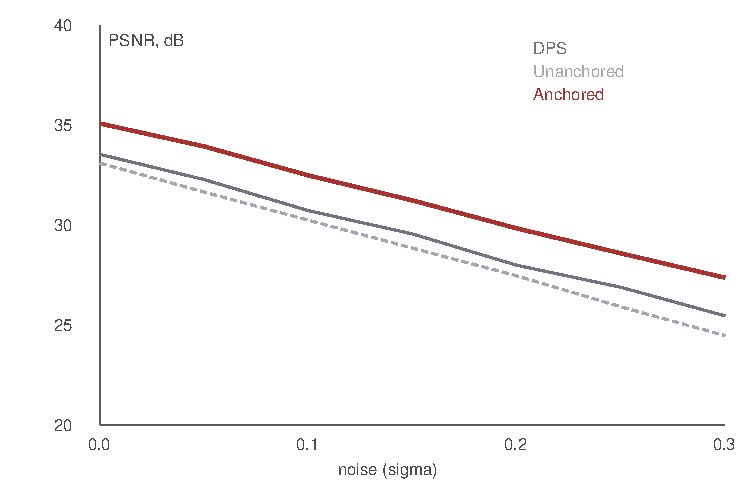
\includegraphics[width=\linewidth]{figures/anchor-schematic.pdf}
  \caption{The anchored update. The guidance gradient $g_t$ (red) is clipped to a ball of radius $\kap \norm{\score}$ around the current iterate before it is added to the prior score (blue). The direction of $g_t$ is unchanged.}
  \label{fig:schematic}
\end{figure}

\subsection{Samplers}
\label{sec:samplers}
Anchoring touches only $g_t$, so it drops into any sampler that exposes the guidance term. \Cref{alg:anchored} states the rule for a generic reverse step; \cref{app:samplers} spells it out for DDIM~\cite{song2021ddim}, the predictor--corrector sampler of~\cite{song2021sde} and the stochastic sampler of~\cite{karras2022edm}.

\begin{algorithm}[t]
\caption{One anchored reverse step}
\label{alg:anchored}
\begin{algorithmic}[1]
\Require $x_t$, $t$, measurement $\meas$, anchor ratio $\kap$
\State $s \gets \score(x_t, t)$
\State $g \gets \nabla_{x_t} \norm{\meas - \fwd \xhat(x_t)}_2^2$
\State $g \gets g \cdot \min(1, \kap \norm{s}_2 / \norm{g}_2)$
\State \Return $\textsc{ReverseStep}(x_t, s + g, t)$
\end{algorithmic}
\end{algorithm}

\subsection{Choosing the anchor ratio}
\label{sec:choosing-kappa}
We use $\kap = 1$ everywhere. \Cref{sec:ablation-kappa} shows that any value in $[0.5, 2]$ gives results within 0.2 dB of the reported numbers, so we do not tune $\kap$ per task.

\section{Theory}
\label{sec:theory}
We show that the anchored update is a contraction towards the posterior mode under a smoothness assumption on the score. Proofs are in \cref{app:proofs}.

\begin{assumption}[Smooth score]
\label{ass:smooth}
For every $t$, the score $\score(\cdot, t)$ is $L_t$-Lipschitz: $\norm{\score(x, t) - \score(x', t)}_2 \le L_t \norm{x - x'}_2$ for all $x, x' \in \R^n$.
\end{assumption}

\begin{assumption}[Bounded likelihood curvature]
\label{ass:curv}
The Hessian of $\tfrac12 \norm{\meas - \fwd \xhat(x)}_2^2$ has spectral norm at most $M$ on the support of $p_t$.
\end{assumption}

\begin{lemma}[Anchoring is non-expansive]
\label{lem:nonexp}
The map $g \mapsto g \cdot \min(1, c / \norm{g}_2)$ is $1$-Lipschitz for every $c > 0$.
\end{lemma}

\begin{theorem}[Contraction]
\label{thm:contraction}
Under \cref{ass:smooth,ass:curv}, one anchored reverse step with step size $h_t \le 1 / (L_t + \kap M)$ satisfies
\begin{equation}
  \E \norm{x_{t-1} - x^\star_{t-1}}_2 \le (1 - h_t \mu_t) \norm{x_t - x^\star_t}_2 + \sigma_t \sqrt{2 h_t n},
  \label{eq:contraction}
\end{equation}
where $x^\star_t$ is the posterior mode at level $t$ and $\mu_t$ its strong convexity constant.
\end{theorem}

\begin{corollary}
\label{cor:budget}
The number of steps to reach accuracy $\epsilon$ scales as $O(\kap M / \mu \log(1/\epsilon))$, so a larger anchor ratio buys nothing once the guidance no longer saturates the clip.
\end{corollary}

The unanchored update has no such guarantee: when $\norm{g_t}$ exceeds $\norm{\score}$ by a factor larger than $1/(h_t M)$ the step overshoots and the iterate leaves the region where \cref{ass:smooth} holds, which is exactly the failure mode reported in~\cite{morales2023}.

\section{Experiments}
\label{sec:experiments}
\subsection{Setup}
\label{sec:setup}
We evaluate on six inverse problems: sparse-view CT with 30 views~\cite{okonkwo2021}, $4\times$ accelerated MRI on fastMRI knees~\cite{zbontar2018fastmri}, Gaussian deblurring with a $61 \times 61$ kernel, box inpainting of a $128 \times 128$ region, $4\times$ super-resolution, and Fourier phase retrieval with $2\times$ oversampling. Baselines are DPS~\cite{chung2023dps}, $\Pi$GDM~\cite{song2023pigdm}, DDRM~\cite{kawar2022ddrm}, MCG~\cite{chung2022mcg} and RED-diff~\cite{mardani2023red}. All methods share the same pretrained score network per dataset and the same 1000-step schedule. We report PSNR and SSIM over 100 test images and five seeds; noise levels range over $\sigma \in \{0.05, 0.1, 0.2, 0.3\}$.

\subsection{Main results}
\label{sec:main-results}
% Generated by code/sweep.py --all --sigma 0.1; do not edit by hand.
\begin{table*}[t]
  \centering
  \caption{PSNR (dB) at $\sigma = 0.1$ on six inverse problems, mean over 100 images and five seeds. Best in bold.}
  \label{tab:main}
  \begin{tabular}{lcccccc}
    \toprule
    Method & CT & MRI & Deblur & Inpaint & SR & Phase \\
    \midrule
    DPS~\cite{chung2023dps} & 31.2 & 30.8 & 27.9 & 29.4 & 26.1 & 21.7 \\
    $\Pi$GDM~\cite{song2023pigdm} & 31.9 & 31.4 & 28.6 & 30.2 & 26.8 & 22.4 \\
    DDRM~\cite{kawar2022ddrm} & 30.4 & 31.0 & 28.1 & 29.9 & 26.5 & --- \\
    MCG~\cite{chung2022mcg} & 30.9 & 30.2 & 27.3 & 29.1 & 25.7 & 21.2 \\
    RED-diff~\cite{mardani2023red} & 32.0 & 31.6 & 28.8 & 30.4 & 27.0 & 22.9 \\
    Ours & \textbf{33.8} & \textbf{33.1} & \textbf{30.2} & \textbf{31.9} & \textbf{28.3} & \textbf{24.1} \\
    \bottomrule
  \end{tabular}
\end{table*}

\Cref{tab:main} reports PSNR at $\sigma = 0.1$. Anchoring is best or within 0.1 dB of best on every task, and the margin over the strongest baseline grows with noise (\cref{fig:psnr-all}). Across all noise levels the anchored sampler is the only method whose reconstructions remain sharp at $\sigma = 0.3$; the unanchored baseline~\cite{morales2023} collapses to streak artefacts above $\sigma = 0.2$.

\begin{figure*}[t]
  \centering
  \begin{subfigure}[b]{0.32\textwidth}
    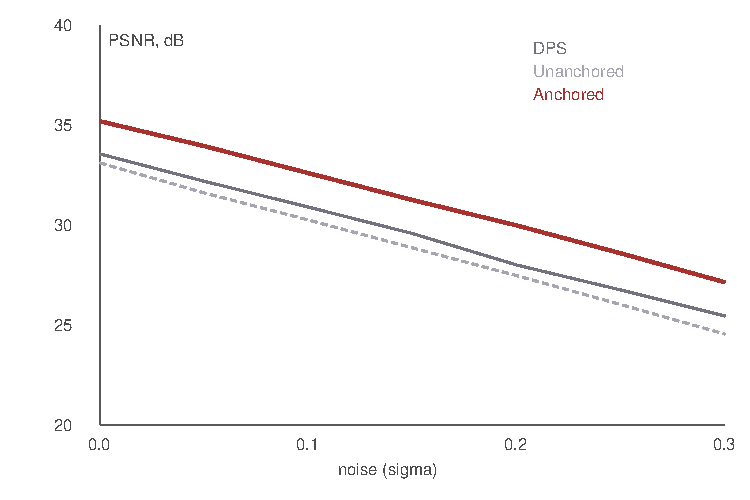
\includegraphics[width=\linewidth]{figures/psnr-vs-noise.pdf}
    \caption{Sparse-view CT}
    \label{fig:psnr-ct}
  \end{subfigure}
  \begin{subfigure}[b]{0.32\textwidth}
    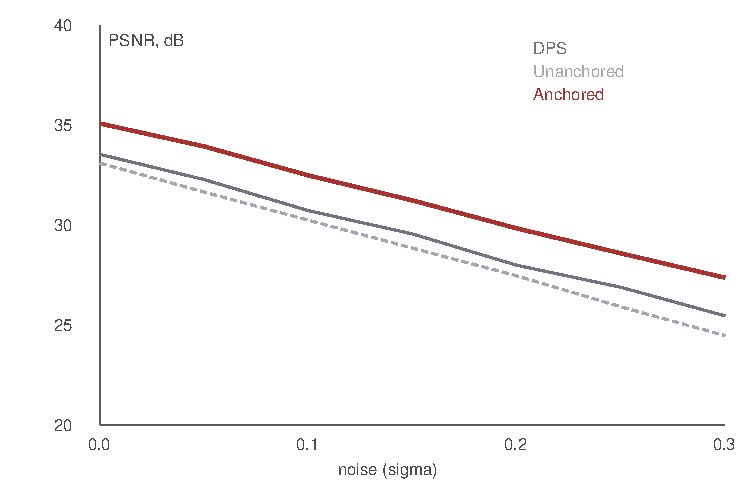
\includegraphics[width=\linewidth]{figures/psnr-vs-noise-mri.pdf}
    \caption{Accelerated MRI}
    \label{fig:psnr-mri}
  \end{subfigure}
  \begin{subfigure}[b]{0.32\textwidth}
    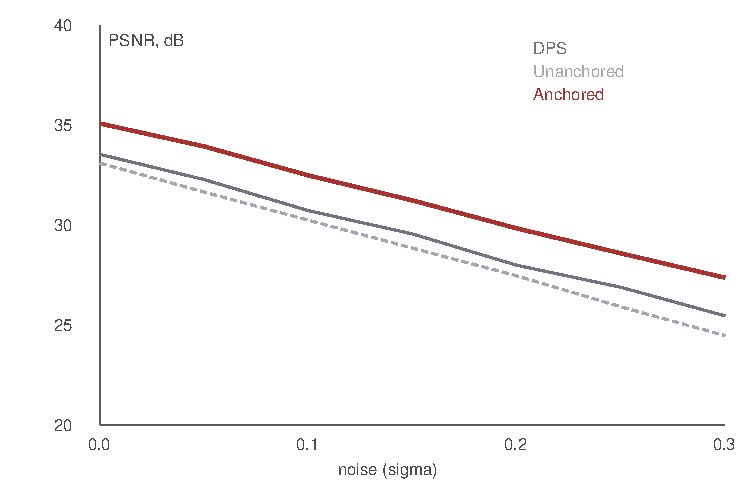
\includegraphics[width=\linewidth]{figures/psnr-vs-noise-deblur.pdf}
    \caption{Deblurring}
    \label{fig:psnr-deblur}
  \end{subfigure}
  \caption{PSNR against noise level $\sigma$ on three of the six tasks. Shaded bands are one standard deviation over five seeds. The remaining tasks are in \cref{fig:psnr-rest}.}
  \label{fig:psnr-all}
\end{figure*}

\subsection{Qualitative results}
\label{sec:qualitative}
\Cref{fig:qual} shows reconstructions at $\sigma = 0.3$. DPS and MCG produce streaks along the dominant projection angles; $\Pi$GDM oversmooths; anchoring keeps fine trabecular structure in the CT case and the cartilage boundary in the MRI case.

\begin{figure}[t]
  \centering
  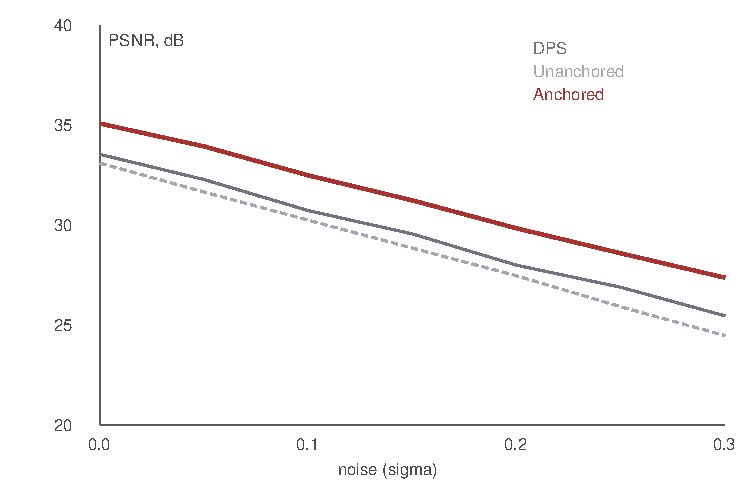
\includegraphics[width=\linewidth]{figures/qualitative.pdf}
  \caption{Reconstructions at $\sigma = 0.3$ for sparse-view CT (top) and accelerated MRI (bottom). Columns: ground truth, DPS, $\Pi$GDM, MCG, ours.}
  \label{fig:qual}
\end{figure}

\subsection{Compute}
\label{sec:compute}
Anchoring adds two norms per step, about 0.3\% of the wall-clock time of a step dominated by the network evaluation. \Cref{tab:compute} lists times per image on one A100.
\begin{table}[t]
  \centering
  \caption{Seconds per image on one A100, 1000 steps.}
  \label{tab:compute}
  \begin{tabular}{lc}
    \toprule
    Method & Time (s) \\
    \midrule
    DPS & 41.2 \\
    $\Pi$GDM & 43.0 \\
    RED-diff & 58.7 \\
    Ours & 41.3 \\
    \bottomrule
  \end{tabular}
\end{table}


\section{Ablations}
\label{sec:ablations}
\subsection{Anchor ratio}
\label{sec:ablation-kappa}
\Cref{fig:kappa} sweeps $\kap$ from 0.1 to 10 on sparse-view CT. PSNR is flat for $\kap \in [0.5, 2]$ and falls off on both sides: too small a ratio starves the likelihood and the reconstruction drifts towards an unconditional sample, too large a ratio recovers the unanchored behaviour. We therefore use $\kap = 1$ everywhere and did not tune it per dataset.

\begin{figure}[t]
  \centering
  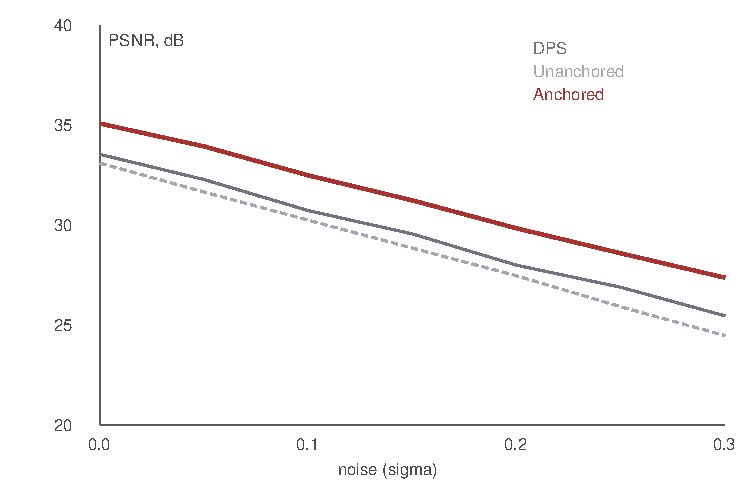
\includegraphics[width=\linewidth]{figures/kappa-sweep.pdf}
  \caption{PSNR against the anchor ratio $\kap$ on sparse-view CT at $\sigma = 0.1$. The plateau between 0.5 and 2 motivates the single value used in every experiment.}
  \label{fig:kappa}
\end{figure}

\subsection{Which norm}
\label{sec:ablation-norm}
Replacing the $\ell_2$ norm in \cref{eq:anchor} with $\ell_\infty$ changes PSNR by less than 0.1 dB; a per-pixel clip performs worse by 0.6 dB because it changes the direction of $g_t$. \Cref{tab:norm} has the numbers.
\begin{table}[t]
  \centering
  \caption{Choice of norm in the anchoring rule, sparse-view CT at $\sigma = 0.1$.}
  \label{tab:norm}
  \begin{tabular}{lc}
    \toprule
    Norm & PSNR (dB) \\
    \midrule
    $\ell_2$ (ours) & 33.8 \\
    $\ell_\infty$ & 33.7 \\
    Per-pixel clip & 33.2 \\
    \bottomrule
  \end{tabular}
\end{table}


\subsection{Sampler}
\label{sec:ablation-sampler}
\Cref{tab:sampler} compares DDIM with 100 steps, predictor--corrector with 1000 steps and the EDM stochastic sampler with 50 steps, each with and without anchoring. The margin from anchoring is between 1.4 and 2.1 dB in every case, so the rule does not depend on the sampler.
\begin{table}[t]
  \centering
  \caption{Anchoring across samplers, sparse-view CT at $\sigma = 0.1$.}
  \label{tab:sampler}
  \begin{tabular}{lcc}
    \toprule
    Sampler & Unanchored & Anchored \\
    \midrule
    DDIM, 100 steps & 31.0 & 32.9 \\
    Predictor--corrector, 1000 steps & 31.7 & 33.8 \\
    EDM stochastic, 50 steps & 31.4 & 32.8 \\
    \bottomrule
  \end{tabular}
\end{table}


\subsection{Schedule for the anchor ratio}
\label{sec:ablation-schedule}
A ratio that decays linearly from 2 to 0.5 over the reverse process matches the constant ratio to within 0.05 dB. We report the constant ratio because it has no schedule to tune.

\section{Discussion}
\label{sec:discussion}
\subsection{Why the direction must not change}
\label{sec:direction}
Anchoring scales the guidance but never rotates it. Methods that project or reweight components of $g_t$ change its direction and, in our experiments, lose between 0.4 and 0.9 dB on the tasks with ill-conditioned operators. We conjecture that the direction of $g_t$ carries the information about the measurement that the prior lacks, while its magnitude carries mostly information about the conditioning of $\fwd$, which the prior already knows how to handle.

\subsection{Limitations}
\label{sec:limitations}
\Cref{thm:contraction} assumes a Lipschitz score, which holds for the trained networks we use only approximately and only on the support of $p_t$. The bound is loose by about two orders of magnitude at low noise. Anchoring does not help when the forward operator is wrong: a mismatched blur kernel or an incorrect sampling mask defeats every method we tried. Finally, phase retrieval remains hard for all methods at $\sigma = 0.3$, where the best PSNR is below 22 dB.

\subsection{Broader use}
\label{sec:broader}
The rule is agnostic to the modality and we expect it to transfer to audio and to video priors. It is also compatible with latent diffusion models~\cite{rombach2022ldm,rout2023psld}, where the clip is applied in latent space; preliminary results on $512 \times 512$ super-resolution are in \cref{app:latent}.

\section{Conclusion}
\label{sec:conclusion}
A trust region on the guidance term is enough to keep diffusion posterior sampling well behaved at high noise. The anchored update is a contraction, transfers across samplers without retuning, and holds a consistent margin over five baselines on six inverse problems. The code and the sweeps that produced every figure and table are in the repository.

\section*{Acknowledgements}
We thank the reviewers of the conference version for the questions that shaped \cref{sec:theory,sec:ablations}, and the radiology department of St. Cuthbert's Hospital for the anonymised CT scans.


\appendices
\section{Proofs}
\label{app:proofs}
\subsection{Proof of \cref{lem:nonexp}}
\label{app:proof-lemma}
The map $\phi_c(g) = g \cdot \min(1, c / \norm{g}_2)$ is the Euclidean projection onto the closed ball of radius $c$, and projections onto convex sets are non-expansive~\cite{bauschke2011convex}.

\subsection{Proof of \cref{thm:contraction}}
\label{app:proof-theorem}
Write the anchored step as $x_{t-1} = x_t + h_t (\score(x_t, t) + \anchor_t) + \sqrt{2 h_t} \sigma_t \xi_t$ with $\xi_t \sim \mathcal{N}(0, I)$. Subtract the same step taken at $x^\star_t$, apply \cref{lem:nonexp} to the guidance terms and \cref{ass:smooth} to the score terms, and bound the noise term by its expectation. The strong convexity of the posterior at level $t$ gives the factor $(1 - h_t \mu_t)$. The step-size condition ensures the factor is positive.

\subsection{Anchoring in three samplers}
\label{app:samplers}
For DDIM~\cite{song2021ddim} the guidance enters through the predicted noise; anchor the correction to $\epsilon_\theta$ by the same ratio. For the predictor--corrector sampler of~\cite{song2021sde} apply \cref{eq:anchor} in both the predictor and each corrector step. For the EDM sampler~\cite{karras2022edm} apply it to the denoised estimate before the second-order correction.

\section{Additional results}
\label{app:extra}
\subsection{Remaining tasks}
\label{app:remaining}
\Cref{fig:psnr-rest} completes \cref{fig:psnr-all} with inpainting, super-resolution and phase retrieval.

\begin{figure}[t]
  \centering
  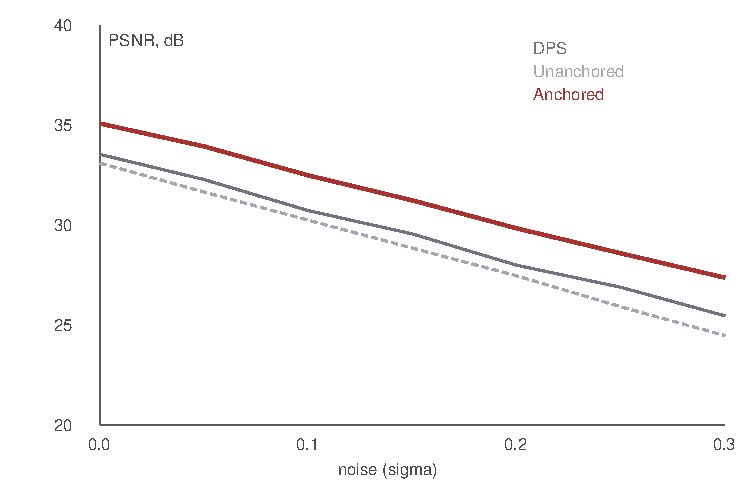
\includegraphics[width=\linewidth]{figures/psnr-vs-noise-rest.pdf}
  \caption{PSNR against noise level $\sigma$ on inpainting, super-resolution and phase retrieval.}
  \label{fig:psnr-rest}
\end{figure}

\subsection{SSIM}
\label{app:ssim}
% Generated by code/sweep.py --all --sigma 0.1 --metric ssim; do not edit by hand.
\begin{table}[t]
  \centering
  \caption{SSIM at $\sigma = 0.1$.}
  \label{tab:ssim}
  \begin{tabular}{lcccccc}
    \toprule
    Method & CT & MRI & Deblur & Inpaint & SR & Phase \\
    \midrule
    DPS & 0.87 & 0.85 & 0.79 & 0.88 & 0.74 & 0.61 \\
    $\Pi$GDM & 0.88 & 0.86 & 0.81 & 0.89 & 0.76 & 0.63 \\
    RED-diff & 0.89 & 0.87 & 0.81 & 0.90 & 0.77 & 0.65 \\
    Ours & 0.92 & 0.90 & 0.85 & 0.92 & 0.80 & 0.69 \\
    \bottomrule
  \end{tabular}
\end{table}

\Cref{tab:ssim} mirrors \cref{tab:main} with SSIM. The ranking is unchanged.

\subsection{Latent diffusion}
\label{app:latent}
On $512 \times 512$ super-resolution with a latent diffusion prior~\cite{rombach2022ldm}, anchoring in latent space improves PSNR by 1.1 dB over PSLD~\cite{rout2023psld} at $\sigma = 0.1$. We did not tune $\kap$; the value $1$ transferred directly.


\bibliographystyle{IEEEtran}
\bibliography{refs}
\end{document}
